%!TEX root = ../main.tex
\section{Homework \thesection}

\subsection{DoG Blob Detection and Scale Selection}
We discussed scale-space ideas and the relationship between the DoG and blob detection.
We will implement these in Matlab and analyze their behavior.
The matlab code provided goes through a sequence of steps.
You will implement three pieces of the algorithm and analyze what is happening on three sample images.\\
The file \href{./hw3/problem1/notes.m}{\texttt{notes.m}} runs through everything.
Probably you only want to use this as reference.\\
The three images that are included are a synthetic image of a circle, a field of sunflowers, and a \emph{brainbow} image of neurons in
a Drosophila brain.
These are depicted below, left-to-right.
The fly-brain is very interesting and a relevant problem for which detecting neuron nuclei is an important problem.
This image has been provided by Dr. Dawen Cai in the Department of Cell and Developmental Biology \href{http://www.cai-lab.org}{\texttt{http://www.cai-lab.org}}.
Each step will run on each image; you are asked to describe what you find and you should do that for each image.
\begin{figure}[htbp]
	\centering
	\begin{subfigure}[t]{0.4\textwidth}
	    \centering
		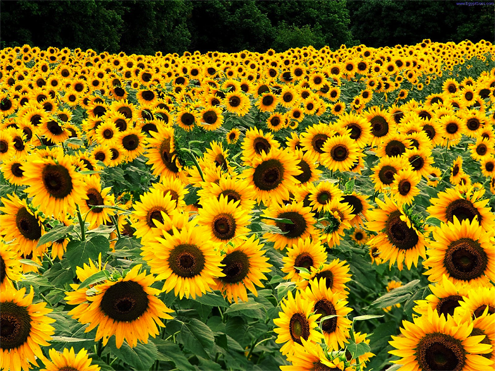
\includegraphics[height=0.2\textheight]{hw3/problem1/sunflowers.png}
		\caption{Sunflowers}\label{fig:10a}
	\end{subfigure}
	\qquad
	\begin{subfigure}[t]{0.4\textwidth}
	    \centering
		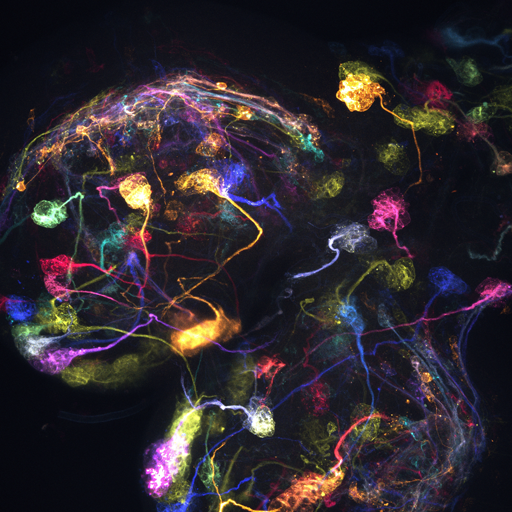
\includegraphics[height=0.2\textheight]{hw3/problem1/drosophila_brainbow.png}
		\caption{Brainbow}\label{fig:10b}
	\end{subfigure}
	\caption{DoG Blob Detection and Scale Selection}\label{fig:10}
\end{figure}
\begin{enumerate}[Step 1]
\item is to create the Difference of Gaussian Scale Space.
		\href{./hw3/problem1/step1.m}{\texttt{step1.m}} is the driver here and it will load/create the images and then call the \href{./hw3/problem1/DoGScaleSpace.m}{\texttt{DoGScaleSpace.m}} function, which you need to implement.
		Follow the instructions in the file and refer to the course notes for how to compute the Difference of Gaussian pyramid.
		Visualization code is included.\\
		Include visualized scale spaces for the sunflower and the circle image in your pdf.
		Describe the scale space and anything you find interesting about it (less than five sentences).
\item is to extract the local extrema of the resulting Difference of Gaussian Scale Space.
		\href{./hw3/problem1/step2.m}{\texttt{step2.m}} is the driver here and it will call the \href{./hw3/problem1/findSSExtrema.m}{\texttt{findSSExtrema.m}}.
		This function looks through \(3 \times 3 \times 3\) windows in space and scale to find local extrema (when the center point is larger or smaller than every other point in the window).
		To ensure you gain the experience of working in a scale space, you may not use the Matlab \texttt{imregionalmax} function.
		Visualization code is included here (called in \href{./hw3/problem1/step2.m}{\texttt{step2.m}}) to visualize the detected extrema.\\
		Provide a visualization of at least the circle-image extrema detections in the scale space.
		Discuss what you see; why are so many extrema detected?
\item is to filter these detected local extrema to reduce the detected set down to a more usable size.
		\href{./hw3/problem1/step3.m}{\texttt{step3.m}} is the driver here and it will call the \href{./hw3/problem1/filterBlobs.m}{\texttt{filterBlobs.m}} function, which you need to fill out.
		This function needs to filter the blobs in two ways.
		First, it needs to filter out blobs that have a DoG response magnitude smaller than a certain threshold (\texttt{DoGtau}), whose value has been provided for fairness.
		Second, it needs to filter out regions that do not resemble blob regions.
		If you carefully inspect the extrema points from the question above, you will find that extrema in the 2D DoG scale space are present in many places other than blobs.
		You need to \textbf{invent a method} for filtering out as many as these extraneous, non-blob-like, extrema as possible.
		You will not be graded on the perfectness of the final method, but you are expected to leverage the methods you know already in the course to accomplish this.
		You should yield filtering results similar in performance to my result below.\\
		Explain your filtering idea, the implementation and the results in your pdf report; include the blob visualizations on the circle and the sunflower image.
		Submission of original code is NOT required.
\item Consider the blob visualization on the drosophila image.
		Include the result blob image here.
		Discuss the detections you find; the false positives; the missing regions.
		Consider the structure of the image.
		Describe an algorithm that could not only find the blobs (cell nuclei) but also the long stringy-things connected to them (cell processes, like axons).
		Can the scale-selection ideas be generalized to lines?
\end{enumerate}

\subsubsection{Difference of Gaussian Scale Space}
The scale space has the property that the higher the level of layer, the less details of the original image.
The output images are in Figure \ref{fig:12}.
The code is from line 32-34, 3 lines only.
\lstinputlisting[style=Matlab-editor]{./hw3/problem1/DoGScaleSpace.m}
\begin{figure}
	\centering
	\begin{subfigure}[t]{0.4\textwidth}
	    \centering
		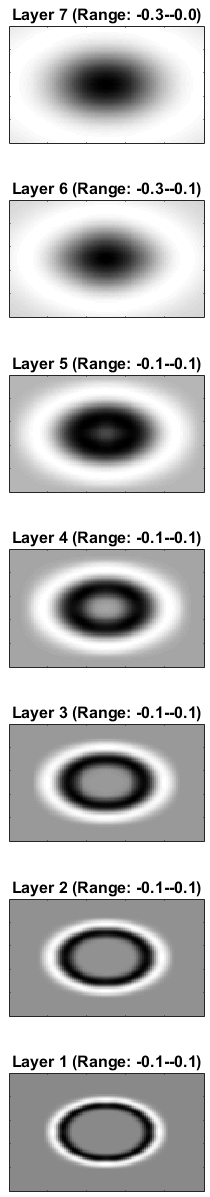
\includegraphics[height=0.92\textheight]{hw3/problem1/DoGSSc.png}
		\caption{\href{./hw3/problem1/DoGSSc.png}{circle}}\label{fig:12a}
	\end{subfigure}
	\qquad
	\begin{subfigure}[t]{0.4\textwidth}
	    \centering
		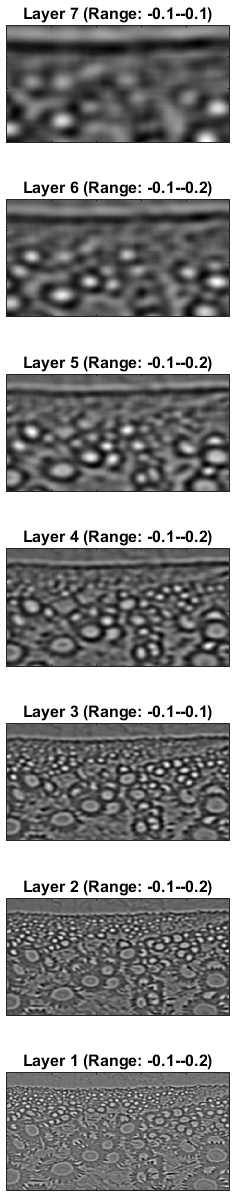
\includegraphics[height=0.92\textheight]{hw3/problem1/DoGSSs.png}
		\caption{\href{./hw3/problem1/DoGSSs.png}{sunflower}}\label{fig:12b}
	\end{subfigure}
	\caption{Difference of Gaussian Scale Space}\label{fig:12}
\end{figure}

\subsubsection{Local Extrema of the Difference of Gaussian Scale Space}
The local extrema are detected in Figure \ref{fig:13}.
The detection on circle image is particularly noisy, because most of the original image have the same value, so the DoG are zero.
Thus, they are treated as extrema.
For the sunflower image, many of the blobs are repeated.
\lstinputlisting[style=Matlab-editor]{./hw3/problem1/findSSExtrema.m}
\begin{figure}
	\centering
	\begin{subfigure}[t]{0.3\textwidth}
	    \centering
		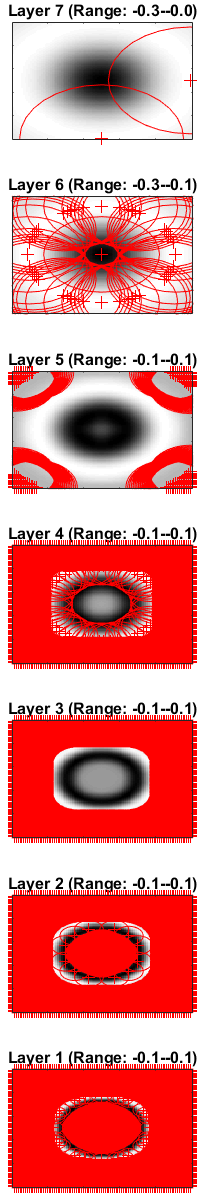
\includegraphics[height=0.92\textheight]{hw3/problem1/SSXc.png}
		\caption{\href{./hw3/problem1/SSXc.png}{circle}}\label{fig:13a}
	\end{subfigure}
	\begin{subfigure}[t]{0.3\textwidth}
	    \centering
		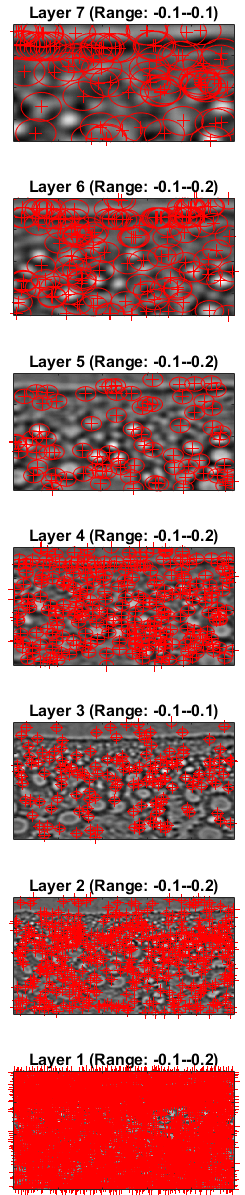
\includegraphics[height=0.92\textheight]{hw3/problem1/SSXf.png}
		\caption{\href{./hw3/problem1/SSXf.png}{sunflower}}\label{fig:13b}
	\end{subfigure}
	\begin{subfigure}[t]{0.3\textwidth}
	    \centering
		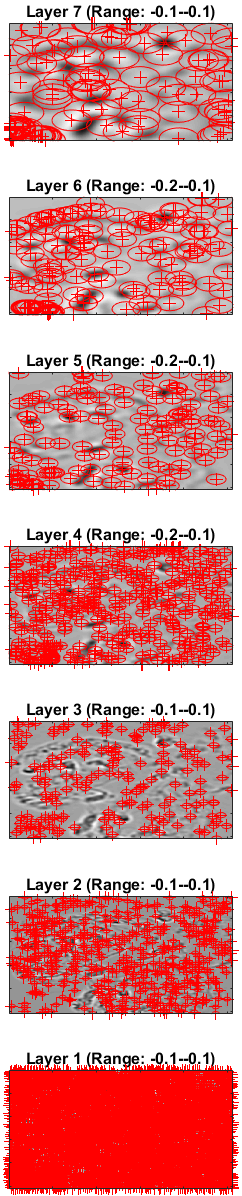
\includegraphics[height=0.92\textheight]{hw3/problem1/SSXb.png}
		\caption{\href{./hw3/problem1/SSXb.png}{brainbow}}\label{fig:13c}
	\end{subfigure}
	\caption{Local Extrema of the Difference of Gaussian Scale Space}\label{fig:13}
\end{figure}


\subsubsection{Filter of Local Extrema of the Difference of Gaussian Scale Space}
The idea of the filtering is to first remove the extrema that has too a response in the Difference of Gaussian.
Then, the non-bolb-like regions are detected by comparing the bolbs.
If two bolbs are too close to each other and the larger one completely covers the smaller one, then the smaller one is expected to be a non-blob-like region.
So we calculate the distances of all pairs of blobs, and if the distance is smaller than the radius of the blob at the higher level, we remove the blob at the lower level.
The results are shown in Figure \ref{fig:14}.
\begin{figure}
	\centering
	\begin{subfigure}[t]{\textwidth}
	    \centering
		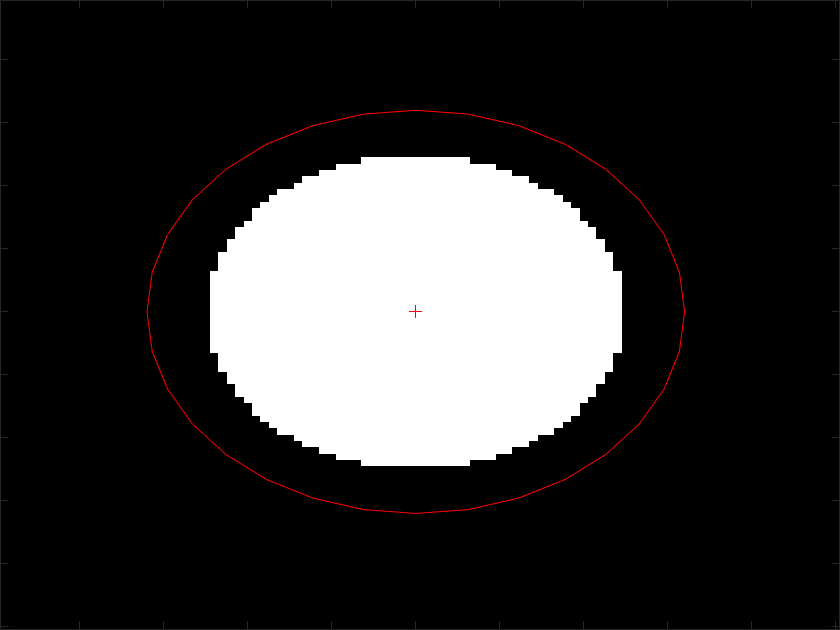
\includegraphics[width=0.84\textwidth]{hw3/problem1/filterc.png}
		\caption{\href{./hw3/problem1/filterc.png}{circle}}\label{fig:14a}
	\end{subfigure}
	\begin{subfigure}[t]{\textwidth}
	    \centering
		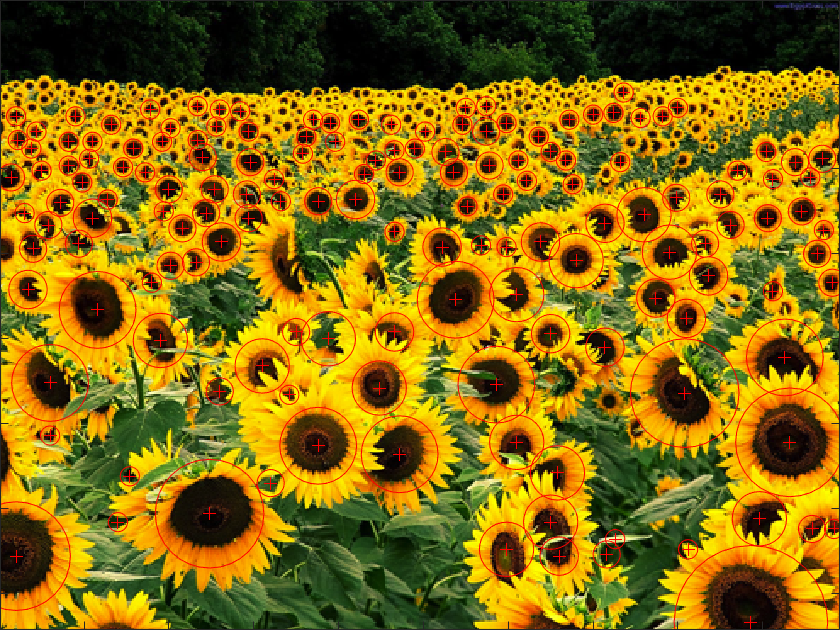
\includegraphics[width=0.84\textwidth]{hw3/problem1/filters.png}
		\caption{\href{./hw3/problem1/filters.png}{sunflower}}\label{fig:14b}
	\end{subfigure}
	\caption{Filter of Local Extrema of the Difference of Gaussian Scale Space}\label{fig:14}
\end{figure}

\subsubsection{Blob Detection on Drosophila Image}
The result blob image is Figure \ref{fig:15}.
Most of the light blobs are detected.
There are very few false positives, and even there are some, they are at the low level layers, so that the sizes of them are small.
There are many missing regions on the right side of the image, since many blobs are too dim, compared with the left side.
One possible algorithm is to combine the blob detection with path searching algorithm.
Starting from one detected blob, we include an adjacent pixel if its intensity is greater than the threshold value.
If the path can finally reach another blob, then the path is found.
This cannot be applied to lines, because a line does not necessarily have blobs at its ends, so the algorithm can't even start.
\begin{figure}
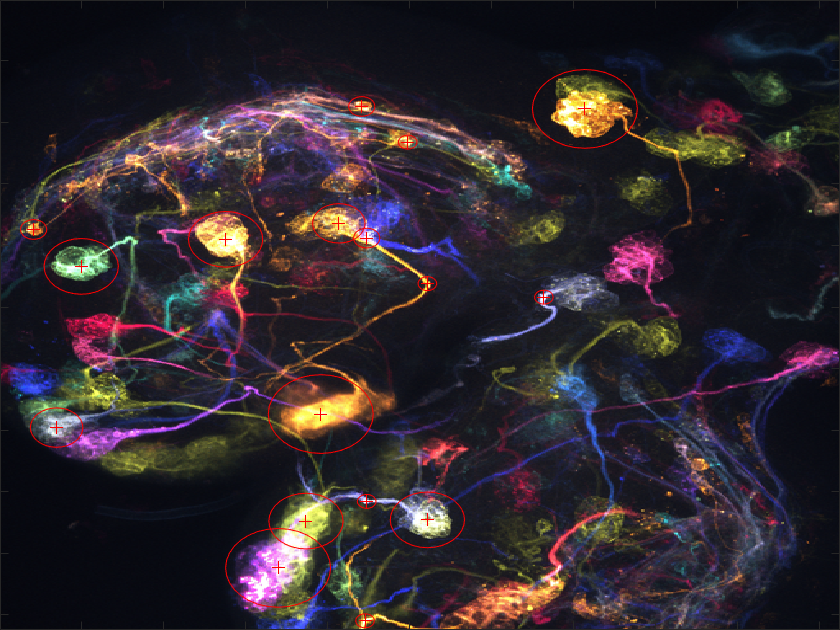
\includegraphics[width=\textwidth]{./hw3/problem1/filterb.png}
\caption{Blob Detection on Drosophila Image}
\label{fig:15}
\end{figure}

\subsection{Matching balloons with SIFT}
We have two images of colorful hot air balloons as shown below, and we want to match the balloons in the two image.
Assume that we've already got the positions of feature points by using some fancy detectors.
To match those feature points in the two images, we need to measure the similarity between points by comparing their feature descriptors.
Since there might be variance in scale, rotation or illumination, SIFT is a good choice to help us complete this task.
\begin{figure}[htbp]
	\centering
	\begin{subfigure}[t]{0.4\textwidth}
	    \centering
		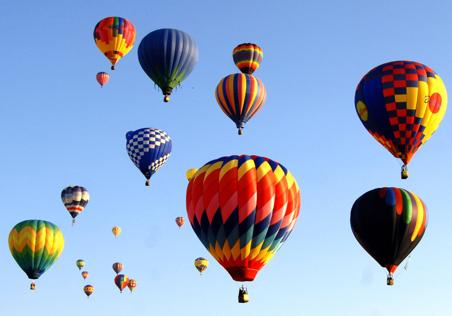
\includegraphics[width=0.8\textwidth]{hw3/problem2/balloons1.jpg}
		\caption{Balloons1}\label{fig:11a}
	\end{subfigure}
	\qquad
	\begin{subfigure}[t]{0.4\textwidth}
	    \centering
		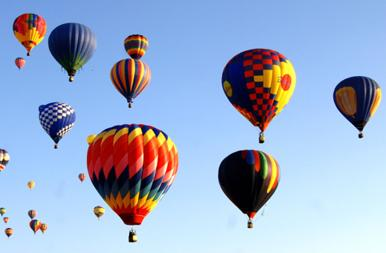
\includegraphics[width=0.85\textwidth]{hw3/problem2/balloons2.jpg}
		\caption{Balloons2}\label{fig:11b}
	\end{subfigure}
	\caption{Matching balloons with SIFT}\label{fig:11}
\end{figure}
Recall the three main steps to do SIFT: localize the feature points, assign orientations and calculate descriptors.\\
To find the scale of the features, you may use \href{./hw3/problem2/DoGScaleSpace.m}{\texttt{DoGScaleSpace.m}} from \textbf{Problem 1} and find the extrema when incrementing the sigma.
Different from \textbf{Problem 1}, you know the exact position of the feature points so just find the scale that gives the strongest response.
To get a good approximation, it is suggested to use smaller increments of sigma and more levels.
One possible set of the parameters is: \(\mathtt{k} = 1.1\), \(\mathtt{s1} = 4*\mathtt{k}\), \(\mathtt{level} = 25\).
It is not the optimal combination.
You can find one set that works for your program.\\
You're provided a list of 5 feature points for each image named \href{./hw3/problem2/points1.mat}{\texttt{points1.mat}} and \href{./hw3/problem2/points2.mat}{\texttt{points2.mat}}.
The main script is \href{./hw3/problem2/matching_balloons.m}{\texttt{matching\_balloons.m}}; it will call the \texttt{sift} function, match the points based on feature descriptors and display the matchings.
Follow the instructions in the script and fill the missing part in \href{./hw3/problem2/sift.m}{\texttt{sift.m}}.
Note that this is a simplified version of SIFT and you're encouraged to learn more about the original algorithm and add more modules into the function.


\lstinputlisting[style=Matlab-editor]{./hw3/problem2/sift.m}